\documentclass[11pt,english,twocolumn]{article}
\renewcommand{\familydefault}{\sfdefault}
\usepackage[T1]{fontenc}
\usepackage[utf8]{inputenc}
\usepackage{pslatex}
\usepackage[english]{babel}
\usepackage{blindtext}
\usepackage{setspace}
\usepackage{url}
% Set the paper size to A4
\setlength{\paperheight}{297mm}
\setlength{\paperwidth}{210mm}
\newcommand{\settextwidth}[1]{
\setlength{\textwidth}{#1}
\setlength{\oddsidemargin}{\paperwidth}
\addtolength{\oddsidemargin}{-\textwidth}
\setlength{\oddsidemargin}{0.5\oddsidemargin}
\addtolength{\oddsidemargin}{-1in}
}
\newcommand{\settextheight}[1]{
\setlength{\textheight}{#1}
\setlength{\headheight}{0mm}
\setlength{\headsep}{0mm}
\setlength{\topmargin}{\paperheight}
\addtolength{\topmargin}{-\textheight}
\setlength{\topmargin}{0.5\topmargin}
\addtolength{\topmargin}{-1in}
}
\addtolength{\topsep}{-3mm}% space between first item and preceding paragraph.
\addtolength{\partopsep}{-3mm}% extra space added to \topsep when environment starts a new paragraph.
\addtolength{\itemsep}{-5mm}% space between successive items.

%End of Simon's mya4.sty
\usepackage{graphicx}%This is necessary and it must go after mya4
\settextwidth{176mm}
\settextheight{257mm}
\usepackage[usenames,dvipsnames,svgnames,table]{xcolor}
\def\baselinestretch{0.95}

\usepackage[compact]{titlesec}
\titlespacing{\section}{0pt}{*1}{*1}
\titlespacing{\subsection}{0pt}{*1}{*0}
\titlespacing{\subsubsection}{0pt}{*0}{*0}
\titlespacing{\paragraph}{0pt}{*0}{*1}
\titleformat*{\paragraph}{\itshape}{}{}{}
%% --------------------------------------------------------------------------------------------------------------------------------
\begin{document}
\title{Automatic Contextual Bug Report Modelling}

\author{Andrei-Mihai Nicolae (2147392)}
\date{}
\maketitle

%====================================================
\section{Research Problem}

\subsection*{Background}

In recent years, software engineering has been shaping many industries that were previously
considered unrelated to technology, ranging from healthcare to public transportation
and education. As software has grown and inflicted itself into so many fields, it has 
inherently become more complex and it now involves teams of even hundreds of developers working
remotely or in the same office on applications that can shape even the face of a nation, such
as Estonia's data exchange layer called X-Road \cite{x-road}.

Therefore, having such a high number of developers working on complex applications, there 
has been a need for software engineers to plan, track and manage the workload for increased 
efficiency. Thus, issue tracking systems have been created, which usually incorporate multiple
components into a single, unified interface. The main component, however, of any issue tracking system
is called a \emph{ticket}. A ticket is comprised of all the necessary information for either
fixing a bug (i.e. specific malfunction of the application) or implementing a new feature 
(i.e. new functionality for the software). However, after an application is released and 
it starts to get used by actual end users, the most common ticket found in issue tracking systems
is a bug report, stating what went wrong inside the application, how it can be reproduced,
even possible locations in the source code where the malfunction might originate from.

Typically, the people who file the bug reports are actual end users who go onto the project's
issue tracking system website and complete the necessary data required by that system. 
Once the bug report is filed in the tracking systen, triagers are responsible for assigning
that ticket to developers to get fixed. Bettenburg et. al \cite{bettenburg2008makes} have 
conducted interviews with developers and they have gathered valuable data related to what
makes for a good bug report and what are the key characteristics that
help them fix the bug as quickly as possible. One result presented by this research is that
having stack traces (i.e. list of methods in the source code which were called when an exception
was thrown) in the description field of the bug report helps developers fix the bug quicker.
However, even with this information available, the fields displayed in the bug report
for the end users to complete (e.g. summary of the bug, description, attachments) are standard
across all the different issue tracking systems.

Having the optimal bug report model/design for end users to complete would be beneficial for both 
the software development team, as well as the overall costs incurred by the company producing
the application. Therefore, the main goal of this proposed project is to create a tool 
that can automatically generate the optimal bug report model for any specific project taking 
into account the characteristics of that project or the team behind it (e.g. size of the
development team, technologies used, mobile/desktop application). Even though there is 
state-of-the-art research in this field, such as the work of Zimmermann et al.\cite{zimmermann2009improving},
they only look into what can be done and propose only advice to issue tracking systems developers.
However, our work goes one step further and we want to conduct the first research in this area
that actually gives the community a tool which can automatically fix this issue.

\subsection*{Key Ideas in a Nutshell}

\emph{"To automatically create a bug report model tailored specifically
for a project, taking into account the whole context of the software as 
well as the developers behind it."}

The goal of the project is to create a tool which, given as input details
regarding the project and the developers working on it, can automatically
generate a bug report model that will increase the efficiency of the team
as well as reduce the costs of the organization. Our proposed approach is to,
firstly, determine what components determine the time-to-fix period (i.e. time spent
between opening a ticket and closing it) for any given project using both
statistical analysis as well as the data already collected in a publicly 
available appendix \cite{breu2009appendix}. 
Then, in order to make our tool take into account all the complex characteristics
of developing software, we want to both look at how the team of developers is 
managed and how the work is distributed, as well as how the developers interact
with the end users reporting the bugs.

The \emph{main benefit} of our project is that, through fixing a still
unresolved issue in the software engineering field, it will improve three 
key aspects:

\begin{itemize}
	\item reduce the overall costs of the organization developing the software;
	\item improve the time-to-fix window for all bug reports, thus reducing
	maintenance effort;
	\item reduce the communication friction between end users and developers
	because having a tailored bug report model will not require engineers
	constantly wasting time on asking for more details from the users reporting
	the bug.
\end{itemize}

\textbf{Example:} The UK government's Health Digital Services department (as well
as many other departments) is using Jira as an issue tracking system \cite{gov-uk-jira}. 
If our proposed application would be used for their project, the developers 
could streamline the bug reports in a timely manner and increase their productivity,
while also decreasing the overall costs for the government.

\subsection*{Objectives}

\subsubsection*{Impact Objectives}

\begin{itemize}
	\item To increase the productivity of software developers in any team
	by giving them bug reports tailored for the project's specific characteristics.
	\item To increase the productivity of managers and triagers as they would
	spend less time on managing the bug reports filed on the issue tracking system.
	\item To decrease the overall costs of the organization financing the software project.
	\item To decrease the level of communication friction between the developers
	and the users filing the bug reports.
\end{itemize}

\subsubsection*{Supporting Objectives}

\begin{itemize}
	\item To present a novel application in the field to the whole research community
	and help advance progress on fixing flaws in major issue tracking systems.
	\item Through making the tool open source, an objective would be to involve
	developers from any industry/academic institution contribute to the advancement of
	this technique.
\end{itemize}

\subsection*{State of the Art}

\emph{Improving Issue Tracking Systems}  The studies of Just et al. \cite{just2008towards} 
and Zimmermann et al. \cite{zimmermann2009improving} have tried to improve the software development
process through analyzing what are the flaws of issue tracking systems and how we can
fix them.

First of all, in the research conducted by Just et al., they asked a large number of
developers about what can be improved about issue tracking systems and ranked the most common
flaws through card sort. They propose a couple of fixes, among which there is better tool support
(e.g. special UI trackers, internationalization),
engage bug reporters in conversations, removing bug report duplicates, as well as improving the
search functionality of issue tracking systems. 

On the other hand, Zimmermann et. al \cite{zimmermann2009improving} propose four areas of 
improvement: tool-centric, information-centric, process-centric and user-centric. The authors
of the study believe that in order to improve these areas, we need to ask end users better 
questions in the bug reports. The solution proposed by the study is the one we want to tackle
in our research and the methodology presented in this paper proved very valuable in designing
our own experiments and evaluation.

\emph{Improving User-Developer Communication} Breu et. al \cite{breu2010information} propose
a rather different approach in their study. They believe that reducing friction between 
developers and end users filing the bug reports would be of great benefit to the software 
development process. They revealed that, because bug reports are not optimized and tailored
to the specifics of the project, the users are not providing the necessary details to the developers,
thus the increased need of engineers continuously discussing with their end users what are the
steps to reproduce the bug, what platform was used when the bug occured etc. This study showed
again that there is a great need from the community for the tool we are developing which would
solve these flaws in the bug reports. 

Another study in this area that looked into a more specific scenario is the one conducted by
Ko et. al \cite{ko2010power}. The authors investigated how projects would benefit if they
centered their bug report design towards more experienced bug reporters, also known as 
\emph{power users}. They show in the study that if issue tracking systems would be more 
focused on them rather than regular users, which file a small number of reports overall, the 
software development process would be greatly improved.

\emph{Personalizing Issue Tracking Systems} In this area, there are two main studies which
propose both advice and prototypes - the research of Baysal et al. \cite{baysal2013situational}
as well as the study conducted by Kononenko et. al \cite{kononenko2014dashboards}. The research
of Baysal et. al \cite{baysal2013situational} proposes a couple of features that could be incorporated into issue tracking
systems that would make them more personalized for the developers, such as private watchers
list (i.e. each developer could privately watch issues without necessarily being CCed on 
every comment or change to the ticket), self tracking (i.e. ability of a developer to track
his own changes and actions for better self management), a patch log, as well as the ability
to assign patch reviewers. These are valuable additions to a issue tracking system that we
believe could help improve the development process. 

Complementing this research, the study from Kononenko et al. \cite{kononenko2014dashboards} 
looks into enhancing developer awareness by proposing a prototype of a issue tracking system
where developers would have their own tailored dashboard to track and manage bug reports in
the project. They admitted some limitations such as the slowness of the application when there
were many queries coming from developers to the servers, but they want to improve the prototype
by adding ElasticSearch \cite{elasticsearch} for running all search queries.

\emph{Simplifying Bug Reports} Herraiz et al. \cite{herraiz2008towards} have investigated
bug reports in the large database of the Eclipse project. Their research concludes that
the standard bug reports from Bugzilla \cite{bugzilla}, which is a popular issue tracking system,
are far too complex and they provide too many fields with too many options to be completed 
by end users, which was found to drive them away from the project and abandoning filing bug 
reports anymore. 

Another study that looked into reducing information needs in issue tracking is the one from
Baysal et. al \cite{baysal2014no}. The authors propose that situational awareness, task 
support and expresiveness are key components in the software development process. They 
conducted a qualitative study where they interviewed a number of software engineers and 
then they proposed a model for bug reports that would facilitate a better functioning for 
task planning and management. 

Covering all this state-of-the-art research, as well as numerous other studies in the field,
there is none that presents a tool which can automatically create bug report models
tailored specifically for any given project.

\subsection*{Our Solution}

In order to tackle automatic contextual bug report modelling, our solution is to first 
create a data mining tool using the recommendations given in the research conducted by 
Kalliamvakou et. al \cite{kalliamvakou2014promises}. We want to scrape bug reports from popular 
open source repositories and analyze their components, as well as infer common patterns. We believe that targeting 
large databases of bug reports, such as the ones from the Mozilla project or the Eclipse project,
will help us gather enough data to make our tool accurate. Moreover, we want to also use the
information available in the appendix created by Breu et. al \cite{breu2009appendix} 
so that we can infer components and possible options available in bug report models from
issue tracking systems.

Then, after scraping all the data and having it available in a database, the next step is
to measure effectiveness of these bug report models so that we can infer what components
or differences in design make the model be more beneficial for the developers. Using the
techniques presented in the works of Bettenburg et. al \cite{bettenburg2008makes} and 
Aranda et. al \cite{aranda2009secret}, we will effectively be able to measure the model's 
effectiveness in the context of the software development process.

After running our analysis on bug report models and their effectiveness, the next step
would be to start developing the tool which will automatically generate the best bug
report model for the project. Firstly, we connect our application to the version control
in order to obtain statistics regarding both the software project as well as the work flows
of the developers. Then, we also hook the tool to the active directory in order to infer the
size of the team, how it is distributed geographically, typical working hours, languages used
etc. Afterwards, we get data from the issue tracking system regarding what type of system it is,
what components and options are available in the bug report model and what can the end user 
reporting the bug see or edit. Finally, we run our tool based on all the data availabe 
and retrieve the best possible design for the bug report, tailored specifically for the project.

Figure \ref{diagram} shows the whole flow that we want 
to apply to our application.

\begin{figure}
	\centering
	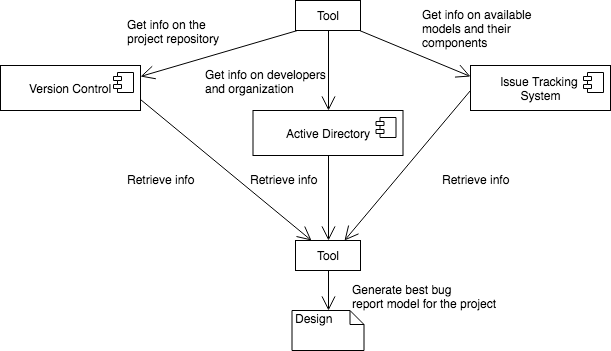
\includegraphics[width=\linewidth]{diagram}
	\caption{Flow of the application}
	\label{diagram}
\end{figure}

As the development of the tool is ongoing, we would like to run the evaluation process in
parallel. We have already discussed with the Mozilla Foundation as well as with the Eclipse
project and they have agreed to let us run the tool once it is available. Firstly, we want to 
conduct interviews with managers, triagers and developers in order to test the validity of
the app and if it actually improves the work flow of the project. Then, we also want to track 
the bug reporters' behavior and see how many abandon reporting the bug, as well as what their
feedback is on the new format.

Finally, we want to publish our application in the open source world as we believe it would
benefit everyone to use it. Moreover, the application could be greatly improved by having 
a large number of experienced developers contributing to it.

\textbf{Example:} Revisiting the Health Digital Services example, they are using Jira as their
issue tracking system. Usinng our tool, we could get all the necessary information to capture
the context and then provide them with the best bug report model so that the software 
development process is improved.

\subsection*{Innovative Aspects}

As we have observed while researching the field, there is no tool that would provide the
same functionality as ours will. Therefore, the biggest innovation of our study is the application
itself which can be used in any project and any issue trackins system. 

Moreover, another innovation that we will bring is that we want to make our tool open source
for the community to be able to contribute. Even though there are other projects who have chosen
the same approach, the number is relatively low - Sonnenburg et. al \cite{sonnenburg2007need} 
conducted a research where they concluded that machine learning, one of the most popular 
areas in the computer science field, suffers from not having many open source tools available
to the community.

%====================================================
\section{Methodology}

\subsection*{Inspection and analysis of bug report models for popular projects (WP1)}

We will first select a handful among the most popular open source projects to scrape.
We have decided that the first two will be the Mozilla and Eclipse projects which also have
their issue tracking systems available to everyone. We will use state-of-the-art techniques
to mine them, such as the ones proposed by Kalliamvakou et. al \cite{kalliamvakou2014promises} 
and German et. al \cite{german2016continuously}. After scraping the issue tracking systems
of these projects, we will then store everything in a database for easy access and ability
to query. 

Then, we will categorize different bug report models based on their components and how
they differ. Also, we will look at the different designs between, for example, Jira and Bugzilla.
Moreover, we want to scrape the project's specific characteristics, such as:
	\begin{itemize}
		\item number of developers and their organization into teams;
		\item technologies used;
		\item geographical and demographics attributes (e.g. geographical position of the 
		developers, languages used);
		\item typical work schedule and work flow of the developers.
	\end{itemize}
\textbf{Deliverables:} data mining tool capable of scraping multiple components, such as 
active directories, version controlled repositories and issue tracking systems; database of
bug report models and their components.

\subsection*{Measure effectiveness for different bug report models (WP2)}

\subsection*{Identity specific components that influenced bug report model effectiveness (WP3)}

\subsection*{Automatically design bug report models optimized per project (WP3)}

\subsection*{Evaluation of the effectiveness of the tool (WP3)}

\subsection*{Identity specific components that influenced bug report model effectiveness (WP3)}

%====================================================
\section{Measurable Outcomes}

%====================================================
\section{Impact and National Importance}

%====================================================
\let\oldbibliography\thebibliography
\renewcommand{\thebibliography}[1]{\oldbibliography{#1}
\setlength{\itemsep}{-3pt}}

\bibliographystyle{abbrv}
%\setstretch{0.8}
{
\scriptsize
\bibliography{proposal}
}
\end{document}
